\documentclass[tikz,border=8pt]{standalone}

\usepackage{amsmath,amssymb}
\usepackage{xcolor}
\usepackage{tikz}

\usetikzlibrary{positioning,arrows.meta,calc,fit,backgrounds}

% Muted publication-style palette.
\definecolor{FNOBlue}{RGB}{70,112,160}
\definecolor{FNOLight}{RGB}{236,243,250}
\definecolor{SSMGreen}{RGB}{76,135,105}
\definecolor{SSMLight}{RGB}{236,247,241}
\definecolor{BaselineGray}{RGB}{118,124,130}
\definecolor{BaselineLight}{RGB}{245,246,247}
\definecolor{RolloutOrange}{RGB}{194,123,55}
\definecolor{RolloutLight}{RGB}{252,243,232}

\begin{document}

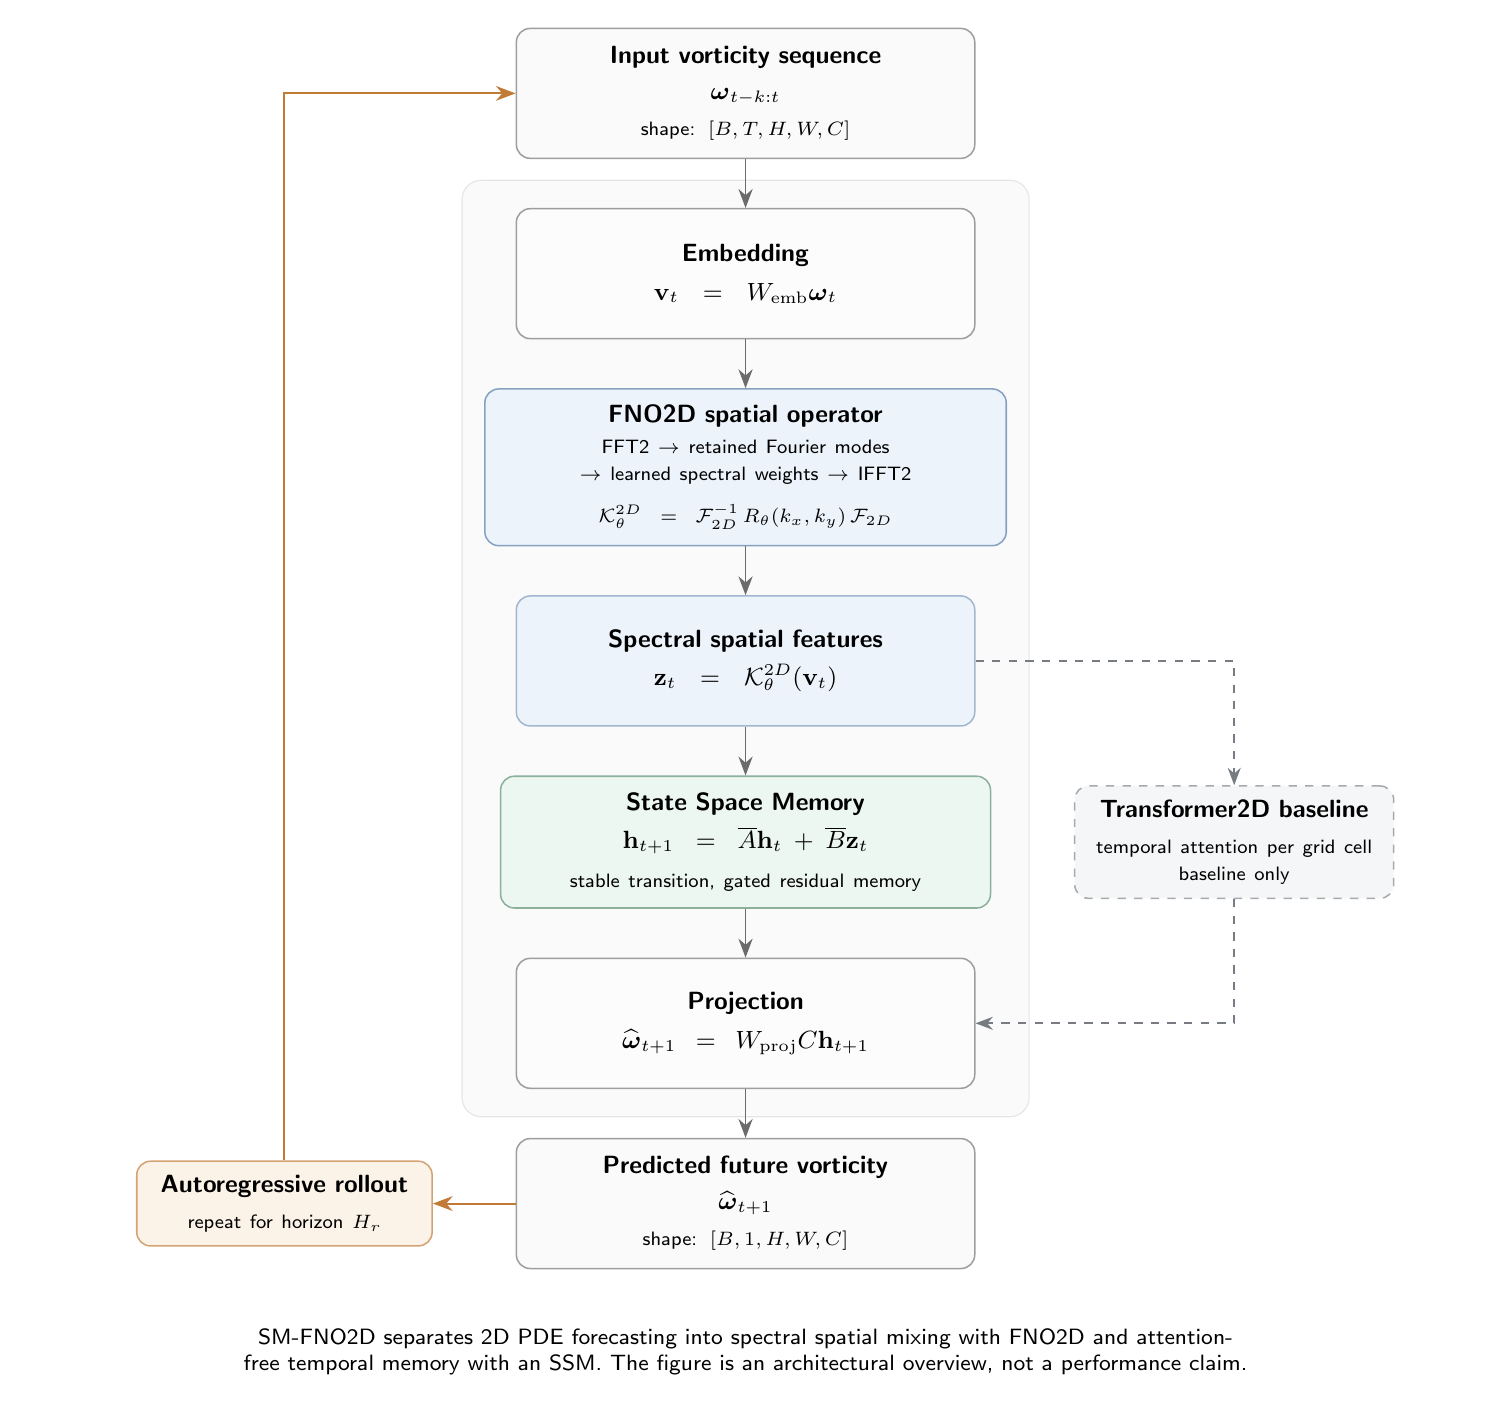
\begin{tikzpicture}[
    font=\sffamily\small,
    >=Stealth,
    node distance=0.62cm and 0.95cm,
    mainarrow/.style={-{Stealth[length=2.4mm]}, line width=0.65pt, draw=black!58},
    rolloutarrow/.style={-{Stealth[length=2.5mm]}, line width=0.75pt, draw=RolloutOrange},
    baselinearrow/.style={-{Stealth[length=2.2mm]}, line width=0.6pt, draw=BaselineGray, dashed},
    block/.style={
        rounded corners=5pt,
        draw=black!38,
        line width=0.55pt,
        fill=white,
        align=center,
        inner sep=6pt,
        minimum height=1.65cm
    },
    inputblock/.style={block, text width=5.4cm, fill=black!2},
    embedblock/.style={block, text width=5.4cm, fill=black!1},
    fnoblock/.style={block, text width=6.2cm, fill=FNOLight, draw=FNOBlue!65},
    featureblock/.style={block, text width=5.4cm, fill=FNOLight, draw=FNOBlue!50},
    ssmblock/.style={block, text width=5.8cm, fill=SSMLight, draw=SSMGreen!65},
    projblock/.style={block, text width=5.4cm, fill=black!1},
    outputblock/.style={block, text width=5.4cm, fill=black!2},
    rolloutblock/.style={
        rounded corners=5pt,
        draw=RolloutOrange!70,
        line width=0.55pt,
        fill=RolloutLight,
        align=center,
        inner sep=5pt,
        text width=3.4cm
    },
    baselineblock/.style={
        rounded corners=5pt,
        draw=BaselineGray!65,
        line width=0.55pt,
        dashed,
        fill=BaselineLight,
        align=center,
        inner sep=5pt,
        text width=3.7cm
    }
]

% Input block: observed vorticity window used by the autoregressive model.
\node[inputblock] (input) at (0,0) {\textbf{Input vorticity sequence}\\[2pt]
$\boldsymbol{\omega}_{t-k:t}$\\[2pt]
{\scriptsize shape: $[B,T,H,W,C]$}};

% Embedding block: channel lift from vorticity values into model features.
\node[embedblock, below=of input] (embed) {\textbf{Embedding}\\[3pt]
$\mathbf{v}_t = W_{\mathrm{emb}}\boldsymbol{\omega}_t$};

% FNO2D block: spatial spectral mixing through a learned Fourier operator.
\node[fnoblock, below=of embed] (fno) {\textbf{FNO2D spatial operator}\\[3pt]
{\scriptsize FFT2 $\rightarrow$ retained Fourier modes\\[-1pt]
$\rightarrow$ learned spectral weights $\rightarrow$ IFFT2}\\[4pt]
{\scriptsize $\mathcal{K}_{\theta}^{2D}=\mathcal{F}_{2D}^{-1}\,R_{\theta}(k_x,k_y)\,\mathcal{F}_{2D}$}};

% Latent feature block: compact spatial representation passed to temporal memory.
\node[featureblock, below=of fno] (features) {\textbf{Spectral spatial features}\\[3pt]
$\mathbf{z}_t = \mathcal{K}_{\theta}^{2D}(\mathbf{v}_t)$};

% SSM block: attention-free temporal state update with stable gated memory.
\node[ssmblock, below=of features] (ssm) {\textbf{State Space Memory}\\[3pt]
$\mathbf{h}_{t+1}=\overline{A}\mathbf{h}_t+\overline{B}\mathbf{z}_t$\\[3pt]
{\scriptsize stable transition, gated residual memory}};

% Projection block: map memory state back to the vorticity channel space.
\node[projblock, below=of ssm] (proj) {\textbf{Projection}\\[3pt]
$\widehat{\boldsymbol{\omega}}_{t+1}=W_{\mathrm{proj}}C\mathbf{h}_{t+1}$};

% Output block: one-step prediction consumed by the rollout loop.
\node[outputblock, below=of proj] (output) {\textbf{Predicted future vorticity}\\[2pt]
$\widehat{\boldsymbol{\omega}}_{t+1}$\\[2pt]
{\scriptsize shape: $[B,1,H,W,C]$}};

% Autoregressive rollout block: predicted states are fed back over the requested horizon.
\node[rolloutblock, left=1.05cm of output] (rollout) {\textbf{Autoregressive rollout}\\[2pt]
{\scriptsize repeat for horizon $H_r$}};

% Baseline branch: secondary comparison path with temporal attention per grid cell only.
\node[baselineblock, right=1.05cm of ssm] (baseline) {\textbf{Transformer2D baseline}\\[2pt]
{\scriptsize temporal attention per grid cell}\\[-1pt]
{\scriptsize baseline only}};

% Background grouping: a light container for the learned one-step forecast map.
\begin{scope}[on background layer]
    \node[
        rounded corners=7pt,
        fill=black!2,
        draw=black!10,
        inner xsep=8pt,
        inner ysep=10pt,
        fit=(embed)(fno)(features)(ssm)(proj)
    ] (modelbox) {};
\end{scope}

% Main top-to-bottom forecast pipeline.
\draw[mainarrow] (input) -- (embed);
\draw[mainarrow] (embed) -- (fno);
\draw[mainarrow] (fno) -- (features);
\draw[mainarrow] (features) -- (ssm);
\draw[mainarrow] (ssm) -- (proj);
\draw[mainarrow] (proj) -- (output);

% Dashed baseline branch, shown as an alternative temporal module without ranking language.
\draw[baselinearrow] (features.east) -| (baseline.north);
\draw[baselinearrow] (baseline.south) |- (proj.east);

% Linear autoregressive feedback path from the one-step prediction back to the input window.
\draw[rolloutarrow] (output.west) -- (rollout.east);
\draw[rolloutarrow] (rollout.north) |- (input.west);

% Short caption kept inside the standalone figure for README and slide export.
\node[
    align=center,
    text width=18cm,
    font=\sffamily\footnotesize
] (caption) at ($(output.south)+(0,-1.05cm)$) {SM-FNO2D separates 2D PDE forecasting into spectral spatial mixing with FNO2D and attention-free temporal memory with an SSM. The figure is an architectural overview, not a performance claim.};

\end{tikzpicture}

\end{document}